\documentclass[12pt]{article}
\usepackage[utf8]{inputenc}
\usepackage{amsmath}
\usepackage{graphicx}
\usepackage{bm}
\usepackage{wrapfig}
\usepackage{footnote}
\usepackage{hyperref}

\bibliographystyle{abbrv} % Choose Phys. Rev. style for bibliograph
\graphicspath{ {../Diagrams/}}

\makesavenoteenv{tabular}

\DeclareMathOperator{\EX}{\mathbb{E}}% expected value

\title{Survey of Data Efficient Approaches to Formality Transfer
\\ \large Advisor: Laura Dietz}
\author{Sean Smith}
\date{Fall 2020\footnote{All code can be found at github.com/sms1097/formality-transfer}}

\begin{document}
\maketitle

\begin{abstract}
    Style Transfer is a problem in Natural Language Processing (NLP) that takes sequences 
    from an input corpus and renders them in the style of a target corpus. The challenge
    of this process comes from creating rewrites in the desired style, while preserving
    content and fluency. One of the major barriers to progress in style transfer is the 
    large data requirements needed to achieve state of the art results. This survey focuses
    on low cost data augmentation and adversarial techniques specifically for the 
    sub-task of Formality Transfer. Unsup-ervised methods are briefly discussed, 
    in addition to the limitations of currently available automatic evaluation metrics. 
\end{abstract}

\section{Introduction}

Style Transfer was introduced in image processing by Gatys et al (2015)~\cite{pictransfer}, 
in which a
content image is rendered in a target style image.  This problem is solved through clever 
manipulation of a cost function that can create impressive re-rendered images. 
\begin{figure}
    \centering
    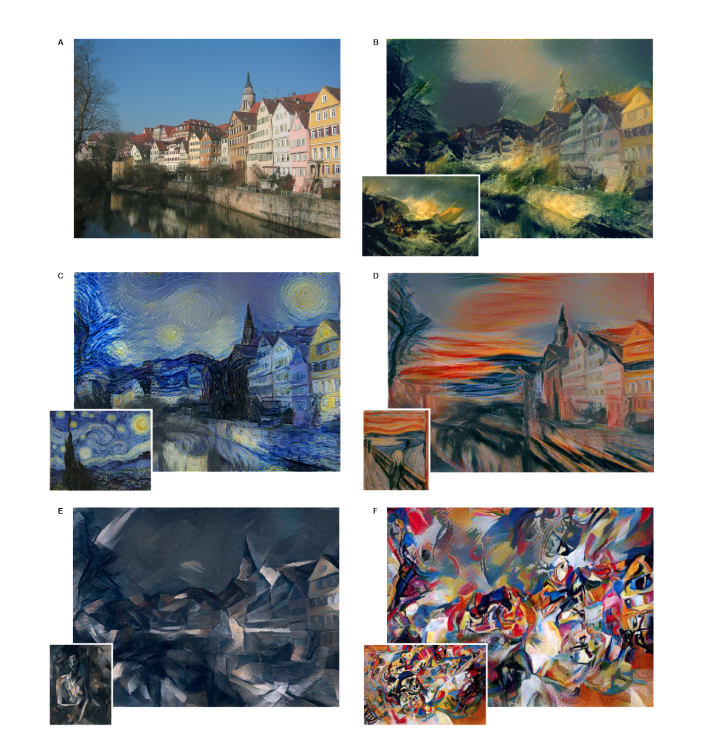
\includegraphics[scale=0.3]{house-painting.png}
    \caption{Example from A Neural Algorithm of Artistic Style}
\end{figure}

Formality Transfer, a specific sub-problem of style transfer, 
typically treated as a Seq2Seq problem and borrows techniques from 
from neural machine translation. This task gained heavy interest from researchers 
with the creation of the GYAFC dataset form Rao and Tetreault~\cite{rao2018dear}.
The GYAFC dataset is a cleaned version of the yahoo L6 corpus~\cite{yahooaaa}. 
Using the L6 corpus Rao and Tetreault had workers translate the informal sequences 
from the corpus to formal rewrites. Two corpora exist, one from the Entertainment and Music category 
and one from the Family/Relationships category. All results included in this report come from the 
entertainment music category

\par One of the biggest barriers to this task, or in general any 
style transfer task, is the lack of parallel data. Machine translation models require large amounts
of data to learn patterns and provide quality rewrites. As a result of this lack of parallel data,
unsupervised methods 
and data augmentation methods are of great interest to researchers currently. 

% Style transfer tasks in NLP stretch a wide variety of applications, the most 
% common of which are Sentiment Transfer and Formality Transfer.
% Other tasks have been explored in research, such as a transfer from technical explan-ations
% to less technical explanations, dubbed Expertise Style Transfer in 
% Cao et al (2020)~\cite{cao2020expertise}.
% Currently each of these tasks has few (albeit not great) automatic evaluation metrics.
% The last section of this review focuses on the shortcomings of current automatic evaluation 
% metrics. 
% \par
% For Sentiment Transfer the new most promising proposed evaluation frame-work is a combination of 
% Word Movers Distance (WMD), Bilingual Evaluation Understudy (BLEU), and Part-of-Speech (POS),
% as proposed in Yam-schikov et al (2020)~\cite{yamshchikov2020styletransfer}. WMD calculates
% the distance between vectors from a learned embedding, so this makes sense for semantic 
% similarity. Yamschikov et al found that this metric was most correlated with scores
% given by human graders too. For four of the datasets assessed in this paper it was found 
% that POS and BLEU were also highly correlated with human grading, however this did not span
% all tasks so the authors recommend using an ensemble of the three metrics.
% \par
% In Formality Style transfer the learning objective is to take informal input and 
% generate formal outputs. Rao and Tetrault (2018)~\cite{rao2018dear} proposed this task 
% and introduced the Grammarly's Yahoo Answers Formality Corpus (GYAFC). 
% Rao and Tetrault use an ensemble of automatic evaluation metrics, similar to what was seen 
% in Yamschikov et al, and also suggested in Pang (2019)~\cite{pang2019daunting}. 
% To assess formality, Rao and Tetreault use an LM perplexity measurement
% suggested in Pavlick and Tetreault (2016)~\cite{pavlick-tetreault-2016-empirical}. 
% Perplexity is the inverse probability of the output sequence normalized by the 
% number of words in the input. To assess perplexity an LSTM model is trained on a 
% formal corpus, specifically in this case English Gigaword. The idea is that 
% informal sentences will be less probable and when evaluated with the perplexity 
% model will have a lower score. The authors also note that a classifier of this 
% nature will need to retrained depending on the domain it is applied to. 
\pagebreak
\section{Supervised Models}

\subsection{Rules with Parallel Encoders}
\begin{wrapfigure}{l}{0.5\textwidth}
    \centering
    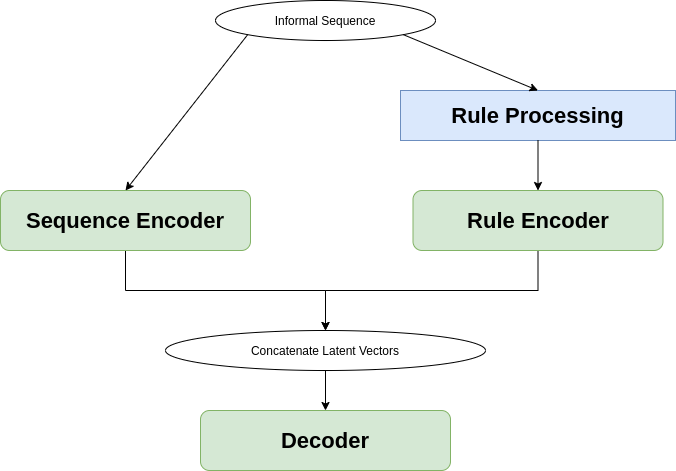
\includegraphics[width=0.5\textwidth]{Rule Concat.png}
\end{wrapfigure}
The approach here is similar to ass-isting a formality transfer model
as shown in Wang et al. (2019).~\cite{rule-harnessing}
Their approach included using rule pre-processing on input sequences and feeding 
a concatenated sequence into two encoders and using hier-archal attention on GPT blocks. \par 
The approach explored here uses the ideas introduced in Chen et al (2018)~\cite{parallelencoders}
by using parallel encoders. The idea here is to feed two sequences in parallel to two different
encoders and then concatenate the hidden states learned by the encoders. \par
For the Transformer
based architecture used by Wang et al. hierarchal attention appears to be the best solution
for formality transfer specifically. Chen at al. found for RNN architectures the concatenation 
of the hidden states gave superior results in machine translation. The concatenation approach
is implemented, in addition to averaging.  

\subsection{Part of Speech Tagging with Parallel Encoders}
This model follows the same paradigm as the Rule based encoder except using part of 
speech labels. A CRF was trained to detect parts of speech on a separate corpus and used 
to create assisted data. This data was then fed through two encoders and their hidden spaces
were concatenated. Two versions of this model were trained, one with concatenated hidden 
states and one with averaged hidden states. 

\section{Semi-Supervised Models}
\subsection{Formality Discrimination}
This technique is covered in Zhang et al (2020)~\cite{paralleldataaug} and involves
augmenting data through a pivot language. In this implementation the training data is translated 
to a pivot language and then translated back. This round trip translation often results in more 
formal sequences which can be used as additional data. \par
Formally we can define our informal corpus as $\mathcal{S}$  with sequences $s$. We can then 
feed $\mathcal{S}$ through our machine translation model to the pivot language, then translate 
the sequence back to english, these round trip translations are denoted $s^\prime$. 
With these re-writes a formality classifier can assign a probability 
of being formal to each sequence. Using the predictions we can define an additional training set 
$\mathcal{T}$ such that 


$$\mathcal{T} = \{(s_i, s_i^\prime)|P_F(s_i^\prime) - P_F(s_i) > \sigma \}$$ 

where $P_F$ is the probability of a sequence being formal. The condition for adding the data
back to the data set is if the round trip translation increased formality by a percent greater
than the parameter $\sigma$. For this implementation a threshold of 0.4 instead of 0.6 as seen
in Zhang et al, as the 0.6 threshold did not increase the data set by a noteworthy result. 
In the end the data set was increased by approximately 8\%. 

\subsection{Backtranslation}
Backtranslation augments data through a reverse training process. This process starts by 
training a machine translation system to do the reverse task of converting formal sequences 
to informal sequences. Modifications to training were performed using techniques discussed in 
Edunov et al. (2018)~\cite{backtranslation}. \par 

For this task random sampling is used of the 
top 10 choices and noise is added to the decoding. Edunov et al. showed that random sampling 
of the synthetic data is much more effective than using a standard beam search for generating data through
backtranslation. The approach used here is to sample the $k$ most likely 
words form the target distribution, re-normalize the new distribution and sample once more. \par


Edunov et al. also showed that introducing noise in the decoding process can 
increase the quality of sequences generated. This technique performs a regular beam-search decoding, but
also introduces dropout, filler token replacement, and deleting words. This technique 
was what was adopted in the training of the model back translation model used in this survey.
\section{Unsupervised Models}
\subsection{Delete, Retrieve, Generate}
Due to the sparsity of data unsupervised models are an active area of research 
in style transfer. One of the first prominent models for semantic transfer without 
parallel corpora comes from Li et al (2018)~\cite{li2018delete}.
Li et al proposed
4 models, each building off of success from other models:
\begin{itemize}
    \item \textbf{RetrieveOnly} returns a randomly selected output sequence $x^{tgt}$.
    This approach will always produce a fluent sentence, but will almost always fail 
    to return a sequence with matching content. 
    \item \textbf{TemplateBased} finds attribute words $a(x, v^{src})$ (where $v_i \in V$
    are the valid style attributes, such as positive or negative) and replaces those words 
    with attributes $a(x^{tgt}, v^{tgt})$. An underlying assumption is that 
    all attribute words appear in the same context, which produces some grammatically 
    incorrect sequences. 
    \item \textbf{DeleteOnly} embeds $c(x, v^{src})$ using an RNN and appends 
    a learned embedding for $v^{tgt}$ and feeds this into a decoder RNN. 
    \item \textbf{DeleteAndRetrieve} embeds $c(x, v^{src})$ and $a(x^{tgt}, v^{tgt})$,
    concatenates both, and feeds this vector into a decoder.
\end{itemize}
\par
Since parallel corpora are not available at training time, the loss function 
for \textbf{DeleteOnly} and \textbf{DeleteAndRetrieve} need to be creative.
\textbf{Delete-Only} is trained by generating new sequences using $c(x, v^{src})$ 
and a target sequence $v^{src}$ in an order to attempt to create a similar sentence 
to the previous one. More formally, we are trying to maximize
$$ L(\theta) = \sum_{(x, v^{src})\in D} \log p(x \, | \, c(x, v^{src}), \, v^{src}; \theta)$$
\textbf{DeleteAndRetrieve} requires more of a rework. With a traditional auto-encoder 
approach the model will learn to recreate the same sentences. The solution is to
introduce a denoising 
auto-encoder which adds a random varia-bility to each of the attribute
words to create $a^{\prime}(x, v^{src})$. The formal definition of the loss function 
becomes
$$ L(\theta) = \sum_{(x, v^{src})\in D} \log p(x \, | \, c(x, v^{src}), \, a^{\prime}(x, v^{src}); \theta)$$

While this problem works well for semantic transfer it fails to generalize 
to formality transfer. All four of the models rely on the salience, which relies 
on n-grams. 
We define an attribute marker $u$ if the salience $s(u,v)$ is 
greater than a threshold $\gamma$. Formally the salience is 
$$ s(u,v) = \frac{\text{count}(u, D_v) + \lambda}{(\sum_{v^\prime \in V, v^\prime \neq v} \text{count}(u, D_{v^\prime })) + \lambda} $$
where $D_v$ is the document of style $v$. The n-gram count in the formal and informal corpora
are both low, and as a result this would not have been a successful implementation for the 
formality transfer task. \par
Using non-parallel corpora, content could be completely lost with no n-gram overlap. In the
formal corpus the most common n-gram appeared only 178 times, and in the informal 441 times.
The most common n-gram in the informal corpus was an accidental double period, which does
provide motivation to the rule based model presented earlier.

% The limitation expressed here does not apply to the previously mentioned retrieval method 
% for the GAN approach. The difference between the retrieval process in the GAN is it is 
% assumed there is a close enough rewrite in the generated data to produce sufficient results,
% which given enough generated data is surely possible. 

\section{Results}
\subsection{Evaluation Metrics}
The following are a brief explanation of the metrics used to assess the models. 
\begin{itemize}
    \item Character n-gram F-score (chrF): 
    $$ (1 + \beta^2) \frac{CHRP \times CHRR}{\beta^2 CHRP + CHRR} $$
    where $CHRP$ is the percentage of n-grams in the predicted sequence that are 
    in the target sequence and $CHRR$ is the percentage of character n-grams in 
    the predicted sequence that are also in the target sequence.  chrF was first 
    introduced by Popovic (2015)~\cite{chrf} to produce a metric that provided 
    better human correlated similarity evaluation than existing metrics. In studies
    Popovic found that chrF provided equal or higher correlation with human evaluation
    as BLEU. 
    \item BiLingual Evaluation Understudy (BLEU): BLEU, first introduced Papineni et al 
    (2002)~\cite{papineni-etal-2002-bleu}, calculates n-gram precision 
    for sequences against the target sequence. 1-4 gram BLEU is calculated as well
    as individual 1-gram BLEU.
    \item  Formality: Formality is calculated by a RNN trained to classify formal 
    sequences on a holdout corpus from the GYAFC dataset. The formality score is 
    the probability the model assigns to the sequence being formal. 
\end{itemize}


\begin{table}[ht]
\caption{Transformer Based Model Results [Bold is significant ($\alpha=0.01$)]}
\centering % used for centering table
\resizebox*{\textwidth}{!}{
    \begin{tabular}{c c c c c} % centered columns (4 columns)
        \hline\hline %inserts double horizontal lines
        Model & BLEU & BLEU (1-grams) & Formality & CHRF \\ [1ex] % inserts table
        %heading
        \hline % inserts single horizontal line
        \underline{Transformer} & 10.38 $\pm$ 0.07 & 30.93 $\pm$ 0.56 & 78.13 $\pm$ 13 & 35.56 $\pm$ 0.89 \\ [1ex]
        Back-Translation & \textbf{10.72} $\pm$ \textbf{0.03} & \textbf{33.59} $\pm$ \textbf{0.23} & 75.68 $\pm$ 0.9 & 9.79 $\pm$ 0.16 \\ [1ex]
        Formality-Discrimination & \textbf{11.78} $\pm$ \textbf{0.07} & \textbf{37.13} $\pm$ \textbf{0.51} & 75.86 $\pm$ 1.53 & 26.73 $\pm$ 0.55\\ [1ex]
        Rule-Assisted & 10.55 $\pm$ 0.04 & 32.2 $\pm$ 0.28 & \textbf{87.56} $\pm$ \textbf{0.43} & 13.12 $\pm$ 0.39 \\ [1ex]
        POS-Assisted & 10.48 $\pm$ 0.07 & 31.68 $\pm$ 0.51 & \textbf{83.19} $\pm$ \textbf{0.98} & 7.9 $\pm$ 0.35 \\ [1ex]
        \hline %inserts single line
        * underlined model is baseline
    \end{tabular}
}
\label{table:nonlin} % is used to refer this table in the text
\end{table}


\begin{table}[ht]
\caption{RNN Based Model Results [Bold is significant ($\alpha=0.01$)]}
\centering % used for centering table
\resizebox*{\textwidth}{!}{
    \begin{tabular}{c c c c c} % centered columns (4 columns)
        \hline\hline %inserts double horizontal lines
        Model & BLEU & BLEU (1-grams) & Formality & CHRF \\ [1ex] % inserts table
        %heading
        \hline % inserts single horizontal line
        \underline{Global Attention} & 10.2 $\pm$  0.07 & 29.51 $\pm$ 0.52 & 1.48 $\pm$ 0.26 & 16.71 $\pm$ 0.29 \\ [1ex]
        Bahdanau Attention & 9.61 $\pm$ 0.07 & 24.93 $\pm$ 0.54 & 1.78 $\pm$ 0.32 & \textbf{26.75} $\pm$ \textbf{0.34} \\ [1ex]
        CRF POS (Concat) & 7.04 $\pm$ 0.02 & 4.88 $\pm$ 0.14 & \textbf{78.49} $\pm$ \textbf{0.52} & 4.63 $\pm$ .07 \\ [1ex]
        CRF POS (Avg) & 7.1 $\pm$ 0.02 & 5.34 $\pm$ 0.14 & \textbf{80.54} $\pm$ \textbf{0.34} & 4.21 $\pm$ 0.14 \\ [1ex]
        Rule Assist (Concat) & 7.6 $\pm$ 0.1 & 9.35 $\pm$ 0.43 & \textbf{67.21} $\pm$ \textbf{0.76} & 3.95 $\pm$ 0.19 \\ [1ex]
        Rule Assist (Avg) & 7.54 $\pm$ 0.04 & 8.77 $\pm$ 0.32 & \textbf{69.47} $\pm$ \textbf{1.62} & 4.31 $\pm$ 0.1 \\ [1ex]
        \hline %inserts single line
        * underlined model is baseline
    \end{tabular}
}
\label{table:nonlin} % is used to refer this table in the text
\end{table}


\begin{figure}[ht]
    \centering 
    \textbf{Transformer Based Model Results}
    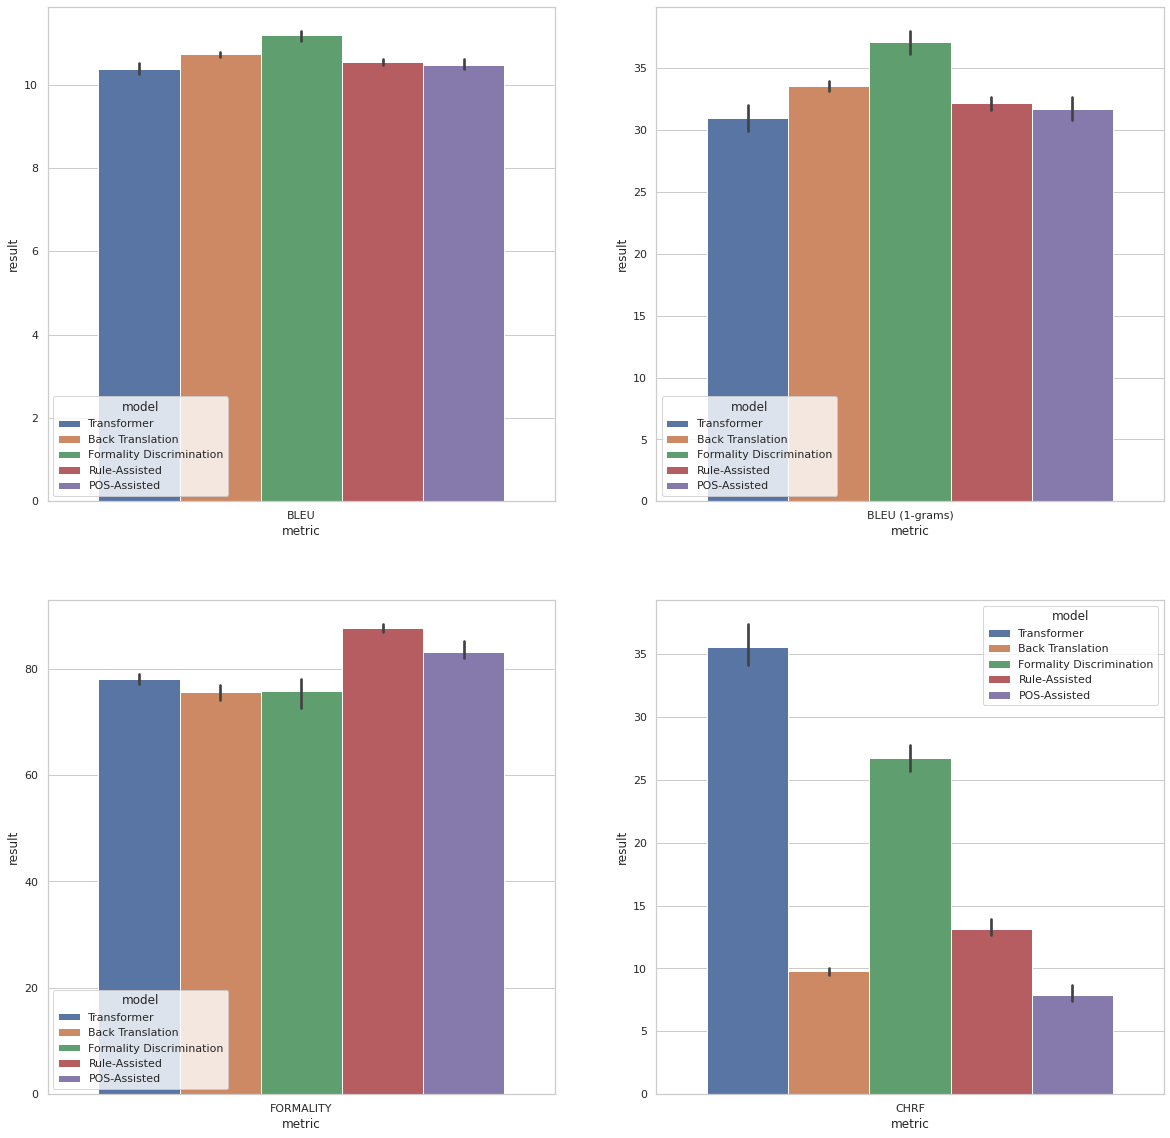
\includegraphics[width=12cm, height=10cm]{transformer-plots.png}
\end{figure}

\begin{figure}[ht]
    \centering
    \textbf{RNN Based Model Results}
    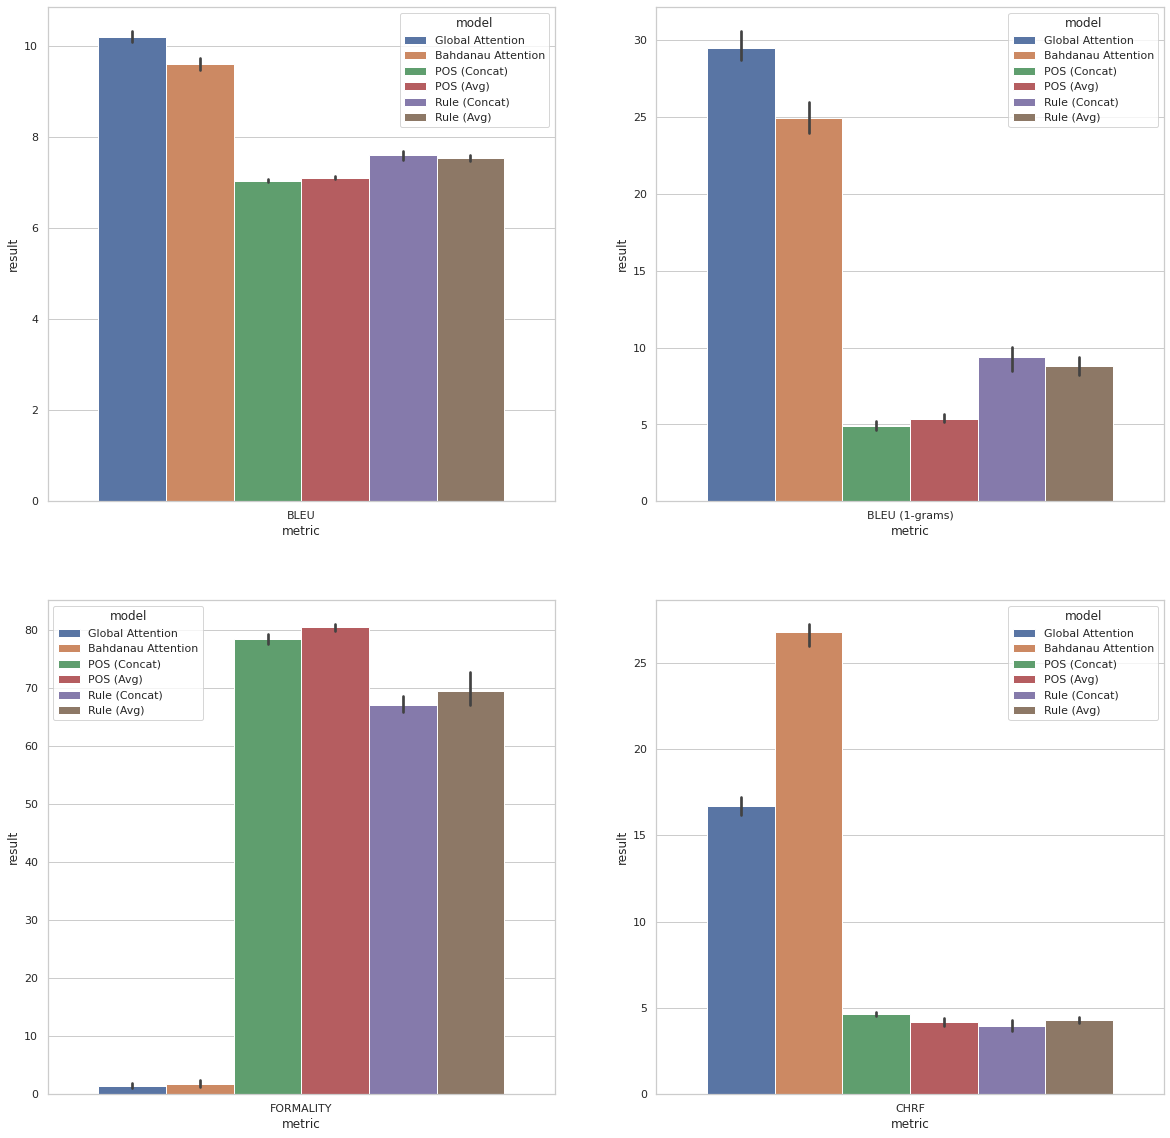
\includegraphics[width=12cm, height=10cm]{RNN-plots.png}
\end{figure}

\subsection{Methodology in Training}
Two base architectures were used in the training of models: Transformers and Attentional RNNs. 
All of the RNN models trained worked form custom implementations of a Seq2Seq model using 
an attention mechanism. The architecture of all models included an embedding initialized with GloVe weights 
and single bidirectional LSTM in the encoder of 1024 units. From there sequences were fed into 
a decoder with a 200 dimensional embedding and an LSTM unit, following into fully connected layers
and an output. All models were optimized using Adam and Sparse Categorical Cross Entropy. All models
used global attention, except for the Bahdanau attention network. \par

The transformer models were trained using OpenNMT-tf. While a custom implemented transformer
was written as part of this survey, the computational requirements to train the model prevented 
practical application of the model. The baseline, backtranslation, and formality Discrimination
models used the prebuilt transformer within the library. The rule-assisted and pos-assisted models
used custom implementations that inherit from the base transformer model. This was done to fit 
the transformer with multi-column encoders. For these transformers, all hyperparameters were 
chosen from Vaswani et al.~\cite{AAYN}

\par
The tables were separated into architecture due to the different origin of the models. The transformers come form the 
OpenNMT-tf library, which is more carfully optimized compared to my implementations. The goal
of the results is to show how using the data augmentation techniques improves the power of
the model. Combing the results into one table and significance testing against a baseline 
either naturally inflates the Transformer models or penalizes the RNN models. 

\par
All models were trained on the same training set consisting of 25,000 sequences and evaluated
on a test set of 2000 sequences. Significance testing was performed by breaking the test group
into 7 groups and computing metrics. A paired t-test between the baseline model and the 
target model was calculated and results that were significantly greater than the baseline model
were recorded. 


\subsection{Model Results}
\par
The Global Attention RNN did not produce nearly as 
good of results. The Global Attention model has significant shortcomings in 
repeated tokens and grammatical errors. The Global Attention model also suffers 
from serious loss of content. Most sequences do not preserve any content whatsoever. \par

The baseline transformer performed well on translations and produced sequences that were mostly
grammatically correct. Upon review most of the sequences retain content strongly while others 
lose some content. An example of this is the translation of the sequence \textit{ray charles is 
the god of smooth music} was translated to \textit{I am streaming music on the job.} While the sequence
is about music, it is more specifically about the legacy of Ray Charles as a musician.  \par

The RNN models aided by part of speech tagging had significant problems in how they learned 
to generate formal sequences. All three of the CRF models did score significantly better 
than their respective baseline model, however they learned to generate sequences that are
nonsensical. These models learned to produce sequences that had excessive punctuation and
capitalized beginning of sentence. For example average sequences resembled 
\textit{They , , , , , , , , , , , , , , , , , , , , , , , , , , , , , , , , , , , , , , , , , , ,}
which is completely nonsensical. It is worth noting that the CRF POS with averaged attention
did test significantly better for BLEU, BLEU (1-grams), and Formality, but it did not actually produce 
sequences that correlated better with human judgements. \par 

The problems seen in the RNN POS assisted models are not observed in the trasnformer rule assisted 
model, but rather a new set of problems were discovered. This model learned to generate sequences that 
are mostly grammatically incorrect. This is largely because the model learned a limited vocabulary of 
149 tokens, most of which are stop words such as \textit{the}, \textit{in}, and \textit{they}. From the 
three part of speech models trained it can be concluded that part of speech does not help increase the 
power of the model and actually appears to hinder the models ability. \par

The RNN Rule assisted models did not perform much better than the CRF models. The rule assisted models
learned similarly to the POS models to capitalize the beginning of sequences. They did not learn 
to use excessive punctuation as seen in the POS models. The sequences generated here learned to create 
partially grammatically correct sequences, but did not learn to finish them (i.e. \textit{Bruce is a} 
or \textit{Yes is} .) This model did appear to converge, which likely indicates that a more complex
model was needed to counteract the issues seen with the model's high variance. \par

The Transformer based rule assisted model produces mostly grammatically correct sequences,
but also mostly loses content in translation. An example of this is the sequence 
\textit{ray charles is the god of smooth music} is translated to 
\textit{I believe the Green Day is playing.} The sequence is mostly correct and the model 
did learn to associate Green Day with music, but completely missed the content of this sequence was 
about Ray Charles. Another example of this is seen in the translation of \textit{hillary's good but
mary-kate and ashley olsen not at all} to \textit{There is a lot of girls, then they are not as well.}
This did learn that the entity names were female but completely missed that the important part of 
the sequence is who the girls actually are. \par 

These sequences were some of models better performances. An example of the model truly underperforming
is the translation of \textit{yO ARE SO UGLY THAT WHEN YOU WHERE BORN YOU 
WERE PUT IN AN INCUBATER WITH TINTED WINDOWS!} was translated to 
\textit{If you do not know , but they should be able to know but they do not know who does not know .}
This is an extreme example of lost content in the model, where complete content is lost. \par 

The backtranslation model achieved a statistically significant result in both BLEU scores, 
however it is one of the worst performing models. In an analysis of the results there 
appear to be no translations that carry content. An example of this is the translation 
is the sequence \textit{Best band: Motley Crue worst: Poison, Stryper( bad christian rock).} 
translated to \textit{I am a Harry Potter movie but not very funny.} Clearly using the data translated 
during backtranslation shows that a focus on producing sequences with good grammar, but terrible transfer
of content. This model may be successful if the amount of backtranslated data was limited to prevent 
the generated sequences from having as much influence over the model as the original sequences. \par 

The formality discrimination model was the best performing model out of all tested. Most of the sequences
maintain content and all are grammatically correct. The downside of this model is it is the most computationally
expensive model to work with, since all sequences need to be translated to the pivot language and back. 
Then after the round trip translation all sequences need to be classified and a threshold for keeping
sequences needs to be tuned. 

\subsection{Discussion of Metrics}

Individual metrics proved to be unreliable in determining success of a model.
Human reviewers were asked to look at a subset of the data from the Bahdanau Attention model
and the Global Attention model to assess fluency, content preservation, and formality. While the 
Global Attention model tested to have significantly better results compared to the Bahdanau Attention model
for both BLEU metrics, these metrics did not correlate with the human reviewers. \par

Rather than making a determination about a model based on one metric, it appears that a good balance of scores 
is needed to assess 
if automatic evaluation of generated sequence align with human reviewers. The best balance seems to be 
between BLEU 
and CHRF, and seeing a lower score in BLEU 1-grams. High BLEU 1-gram scores with low BLEU scores tended 
to indicate models did not learn to produce well rounded sequences. If the model
can only learn 1-grams then likely meaning is being lost. The balance between BLEU and CHRF allows
to evaluate how many n-grams are matching, but also how many subsets of words are matching. For example
if the model translates a word with the wrong tense, CHRF can see it is still attempting to learn 
the correct content transfer, but did not achieve the correct fluency. This kind of translation mistake
may not bother human reviewers, but would penalize the sentence greatly in BLEU scores. \par

The idea of aggregating metrics is suggested in Pang (2019)~\cite{pang2019daunting}, where a weighting
scheme could be enforced on the metrics to find a combination that is correlated with human judgement. 
The procedure for creating such a metric would involve taking outputs from many models and randomly sampling 
sequences to show to reviewers. After review, a new metric could be trained on the results of human 
review. A limitation of this metric is that the aggregation would not necessarily 
translate between data sets. In order to achieve a universal metric, outputs from many models trained on 
different data sets would need to collected and reviewed. 

\par
Another interesting takeaway is the sensitivity of the Formality metric. The model was trained to 
achieve 91\% accuracy on a holdout set that also comes from the GYAFC corpus. 
In training, a jump from 80\% to 91\% was achieved simply from preventing the tokenizer from 
only learning lowercase representations and tokenizing the period character. 
This likely indicates that the biggest factors in what the neural network is learning comes from 
complete sentences, since the primary repeated token is a period. The classifier also learned to 
favor sentences as formal when they began with a capitalized letter. 


\section{Future Work}
\subsection{Data Augmentation with Seq2Seq GAN}
\begin{figure}[t]
    \centering
    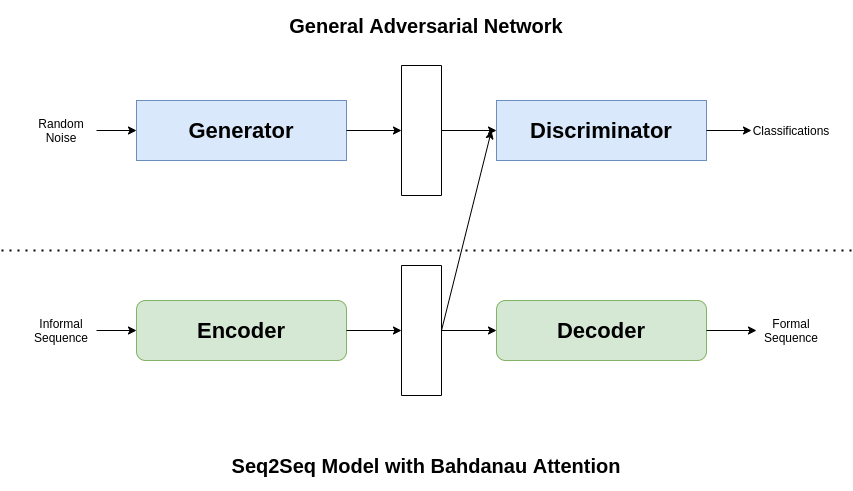
\includegraphics[scale=0.4]{GAN Generation.png}
\end{figure}

This adversarial approach has not been used before in formality transfer, but seems 
to have some potential. This approach is based on ideas expressed in 
Donahue et al (2018)~\cite{ganpaper}. A Seq2Seq model is trained 
using available parallel data until minimally acceptable results are achieved.
A generator is then fed random noise to create tensors that are equal in size to the 
intermediate tensor in between the encoder and decoder. The discriminator is fed both 
tensors and attempts to distinguish between which sequences are real and which are fake. 
The generator is rewarded for fooling the discriminator and the discriminator is rewarded
for detecting the generator outputs. Training is stopped once the discriminator is no 
longer able to distinguish if a tensor came from the generator of the Seq2Seq model. \par 

It is important to distinguish that the GAN must be trained on the intermediate sequence
instead of output sequences or tokens. When training the GAN we are essentially playing a 
minimax game, such that the loss of the Discriminator is maximized while the loss of the
generator is minimized. In a normal RNN architecture, the network is trained to minimize 
cross entropy with the target token at the step of a sequence. With this minimax algorithm 
the new goal for the RNN is to minimize the loss of the discriminator. When iterating 
through the sequence and choosing the most likely token, we were performing an operation 
that was not differentiable, since the loss was calculated according to how well that token
matched. In order to be able to apply a loss function to the discriminator, we need a 
differentiable operation, and we can achieve this by learning to generate the intermediate
sequence between the encoder and decoder.  


Using the GAN we can generate useful data in two ways. First a pre-trained
back translation model could be used to generate informal sequences form the 
formal sequences. The upside of this approach is the potential for unlimited data, however
there exists potential problems with the balance of generated data and original data. 
The quality of the data should not matter for the translation process, since the sequences
created by the backtranslation in the formal to informal are of relatively poor quality, but
the informal to formal sequences achieve great fluency. This of course assumes a successful 
convergence of the GAN. \par

The second approach for using GAN data is using similarity metrics between
the informal corpus and generated sequences to pair rewrites. Jacc-ard similarity is
a retrieval metric which
computes the intersection over union for sequences. In trials this mostly returned 
correct sequence pairs between formal and informal sequences. 
Another is cosine similarity, which computes distances between vectors representing
term counts. Similarly to Jaccard similarity this metric could be used to retrieve 
sequences form the generated sequences that are close to the informal sequences. A minimum
distance could be selected based upon results. \par

Due to time and resource constraints this GAN approach could not be fully developed.
Further experimentation needs to be done to produce a GAN that can generate 
adequate data. All implementations that currently exist suffer from mode collapse. 
Different combinations of additional noise, learning rate tuning, and label smoothing 
were attempted, but with no success.
Likely the current approach will not prove to be adequate and a pure autoencoder
would need to be trained. In exper-imentation, it was difficult to find an autoencoder
that produce sequences of high enough quality for the generation to be worth 
pursuing. This approach might also require expanding the data set with the other half
of the supervised corpus. 

\subsection{Entity Transfer Metric}
As seen in many of these sequences while some content was transfered while important 
distinguishing features, such as prominent figures, were lost. This does motivate exploration
of a metric that can detect the transfer of entities form one sequence to another, and harshly
penalize sequences that lose entities. This could also be explored at the model level
to find ways that entity transfer can be enforced in the translations. 

\section{Conclusions}
Style transfer is a great upcoming field in NLP that has seen 
considerable amounts of clever research and still has great room for potential.
This survey showed novel experimental ideas for style transfer stemming from machine 
translation. The shortcomings of current evaluation metrics was also shown. Areas for 
future research were presented based upon the results from implemented models, including 
experimental data augmentation strategies and evaluation metrics. 

\pagebreak
\bibliography{qhe}
\end{document}